\chapter{Modelos de neurônio}\label{cap:modelos}
\section{Introdução}\label{sec:modelos_intro}
Os modelos são formas de representar, matemática e/ou computacionalmente, o comportamento do neurônio. Os modelos podem variar desde os mais simples, que não representam fielmente o comportamento fisiológico do neurônio mas são úteis para simular grandes quantidades de neurônios, até os mais complexos, que trazem diversas representações de condutância e morfológicas. Alguns modelos de neurônio são apresentados na Tabela~\ref{tab:modelos_neuronios}, incluindo o número de variáveis presentes no modelo, o que reflete o número de equações diferenciais presentes e, consequentemente, a complexidade do mesmo, bem como é informado se o modelo é considerado biologicamente plausível. Os 4~(quatro) primeiros modelos são detalhados neste texto, por hora diferenciados entre os que simulam o disparo do potencial de ação, chamados aqui de modelos de disparo de neurônio, e os que simulam a taxa de disparo. Há, ainda, distinção, por exemplo, entre modelos de compartimento único, que modelam o potencial de membrana apenas pela variável $V$, e os multi-compartimento, que consideram variações espaciais no potencial de membrana, porém estes últimos não são abordados neste texto.

\begin{table}
	\centering
	\caption[Modelos de neurônio]{Modelos de neurônio}
	\label{tab:modelos_neuronios}
	\begin{tabular}{|c|c|c|c|}
		\hline
		Modelo & N. variáveis & Complexidade & Biol. plausível \\
		\hline
		Leaky integrate-and-fire & 1 & Muito baixa & Não \\
		\hline
		Izhikevich & 2 & Muito baixa & Não \\
		\hline
		Hodgkin-Huxley & 4 & Muito alta & Sim \\
		\hline
		Wilson-Cowan & 2 & Média & Não \\
		\hline
		Spike response model & 1 & Baixa & Não \\
		\hline
		FitzHugh-Nagumo & 2 & Média & Não \\
		\hline
		Moris-Lecar & 3 & Alta & Sim \\
		\hline
	\end{tabular}
\end{table}

\section{Modelos de disparo de neurônios}\label{sec:modelosdisparo}
\subsection{Modelo integra-e-dispara com vazamento}\label{sec:modelolif}

Para modelos de neurônio de compartimento único, o circuito elétrico equivalente da membrana pode ser representado como na Figura~\ref{fig:circuitomembrana}.
\begin{figure}[htb!]
	\centering
	\caption{Circuito equivalente da membrana}
	\label{fig:circuitomembrana}
	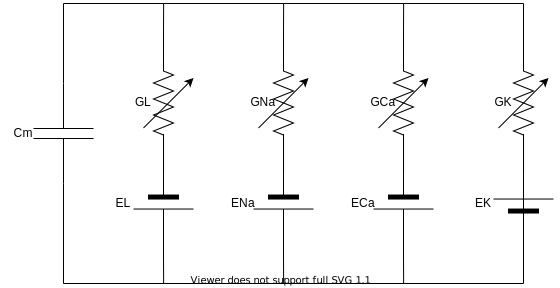
\includegraphics[width=0.7\linewidth]{figs/circuito_membrana}\\
	\cite{lapicque_recherches_1907}
\end{figure}
O capacitor na esquerda está associado à capacitância da membrana ($C_m$), e cada resistor em série com uma bateria representa um canal iônico. A série com o $L$ subscrito refere-se ao elemento de vazamento, citado anteriormente, e as séries são referentes aos canais iônicos dependentes de tensão, com o íon subscrito. O circuito completo tem associada a seguinte equação:
\begin{equation}\label{eq:potencial_membrana_total}
	c_m\frac{\mathrm{d}V_m}{\mathrm{d}t}=G_{Na}(E_{Na}-V_m)+G_{Ca}(E_{Ca}-Vm)+G_K(E_K-V_m)+G_L(E_L-V_m)
\end{equation}
sendo $G_A$ a condutância do íon $A$, $E_A$ o potencial do íon $A$. Ignorando por hora os canais iônicos dependentes de tensão, a equação fica como a \ref{eq:potencial_membrana}. Adicionando-se a corrente aplicada, incluímos também uma condição que força o disparo do potencial de ação quando o potencial de membrana atinge um determinado limitar ($V_{th}$), forçando o potencial de membrana para um valor de \textit{reset} ($V_{reset}$) \cite{miller_introductory_2018}. Com isso, o circuito fica equivalente à Figura~\ref{fig:circuitolif} e a equação total é como abaixo.
\begin{equation}\label{eq:lif}
	c_m\frac{dV_m}{dt} = G_L(E_L-V_m)+I_{ap}; \text{ se } V_m > V_{th} \text{ então } V_m\mapsto V_{reset}
\end{equation}
\begin{figure}[htb!]
	\centering
	\caption{Circuito equivalente do modelo LIF}
	\label{fig:circuitolif}
	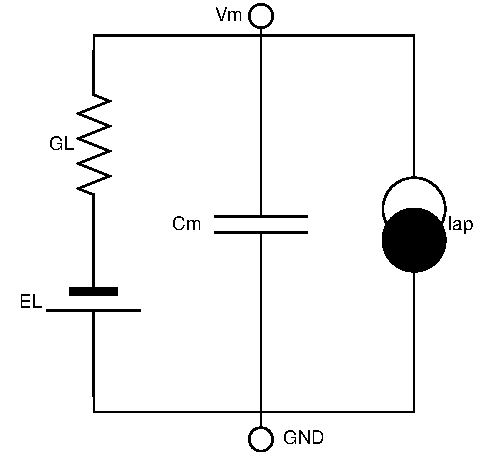
\includegraphics[width=0.5\linewidth]{figs/circuito_lif}
\end{figure}
Essa é a equação do modelo \textit{Leaky integrate-and-fire} (integra e dispara com vazamento, em tradução livre). A corrente aplicada no modelo é acumulada (integrada), elevando o potencial de membrana até o valor de limiar, representando o momento onde o neurônio dispara. Devido a simplicidade do modelo, a equação, por si só, não é capaz de representar a hiperpolarização que ocorre fisicamente na célula neuronal após o disparo do potencial de ação, e, por isso, é acrescentada a condição de \textit{reset}. Enquanto a corrente continuar sendo aplicada, o potencial de membrana permanece sendo atualizado pela dinâmica da equação diferencial, como é exibido na Figura~\ref{fig:lif}. Três pulsos de corrente, com valores $0,18\ nA$, $0,21\ nA$ e $0,24\ nA$, são aplicados no modelo. Para o primeiro valor, o neurônio despolariza (fica menos negativo), porém não atinge o valor de limiar (como visto na primeira curva da segunda linha de gráficos). Com a injeção dos demais valores de corrente, a célula neuronal atinge o valor de limiar ($50\ mV$ nestes exemplos), ocorrendo o disparo do potencial de ação (registrado como uma linha vertical na última linha de gráficos), e com a posterior alteração do potencial de membrana para o valor de \textit{reset} ($80\ mV$ nestes exemplos).

\begin{figure}[htb!]
	\centering
	\caption[Exemplo da simulação com o modelo LIF]{Exemplo da simulação com o modelo LIF. Cada coluna representa um valor diferente de corrente aplicada ao modelo, que são mostradas na primeira linha de gráficos. Na segunda linha são exibidos os potenciais de membrana para cada corrente injetada. Em baixo, os instantes em que ocorreu o disparo de potenciais de ação.}
	\label{fig:lif}
	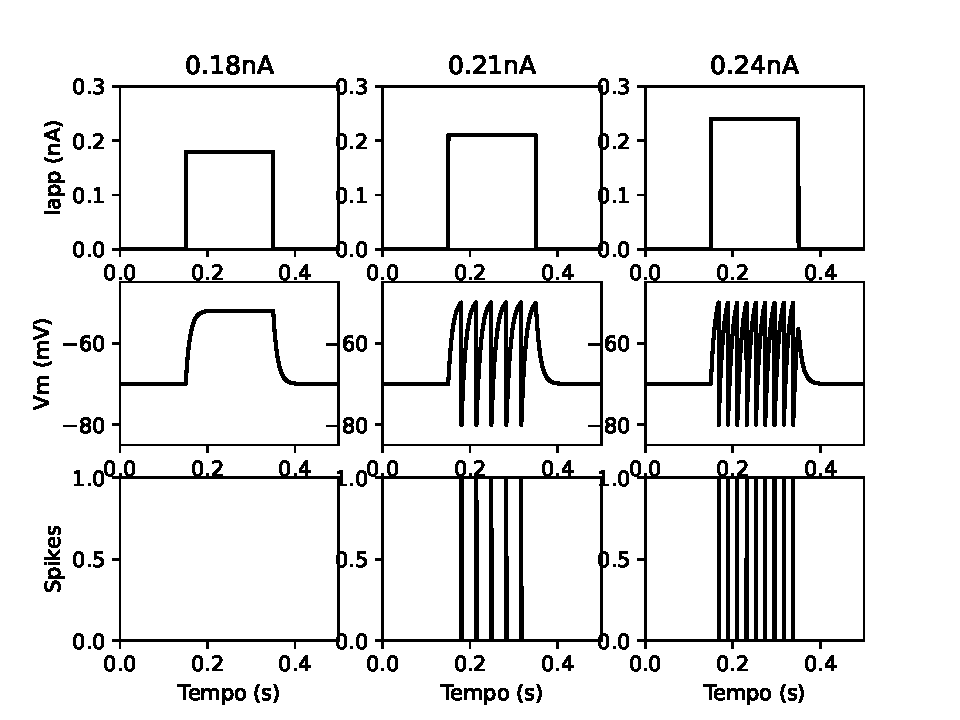
\includegraphics[width=0.7\linewidth]{figs/lif}
\end{figure}

%% incluir a solução analítica para enfatizar a presença da constante de tempo

\subsection{Extenções do modelo LIF}

\subsubsection{Período refratário}
Imediatamente após a ocorrência do potencial de ação, o neurônio não é capaz de produzir um novo potencial de ação durante um curto período de tempo, e esse tempo é chamado de período refratário. Existem diferentes maneiras de simular o período refratário nos modelos neuronais, e aqui mostramos três acrescentadas ao modelo LIF

\begin{description}
	\item[Grampeamento de tensão] Trata-se de fixar o valor do potencial de membrana no valor de reset durante um tempo específico logo após o potencial de ação
	
	\item[Condutância refratária] Este método acrescenta uma condutância elevada, que gera uma corrente de potássio hiperpolarizante, cresce imediatamente após cada potencial de ação, e decai seguindo a seguinte equação diferencial:
	
	$
	\frac{dG_{ref}(t)}{dt} = -\frac{G_{ref}(t)}{\tau_{ref}};\text{ depois do potencial de ação } G_{ref} \mapsto G_{ref} + \Delta G
	$
	
	sendo $\tau_{ref}$ a constante de tempo do período refratário e $\Delta G$ o incremento de condutância. A corrente de potássio é representada acrescentando-se à parte direita da equação do modelo LIF o termo $G_{ref}(t)[E_k-V_m(t)]$, com $E_k$ sendo o potencial de Nernst para íons de potássio
	
	\item[Incremento do limiar] Este método eleva, após cada potencial de ação, o limiar necessário para produzir um novo potencial de ação, e esse limiar decai seguindo a seguinte equação diferencial:
	
	$
	\frac{dV_{th}(t)}{dt} = \frac{V^0_{th}-V_{th}(t)}{\tau_{ref}};\text{ depois do potencial de ação } V_{th} \mapsto V_{th} + \Delta V
	$
	
	sendo $V^0_{th}$ o potencial de limiar de referência
	
	\begin{figure}[htb!]
		\centering
		\caption{Simulação do modelo LIF com período refratário}
		\label{fig:lifrefratario}
		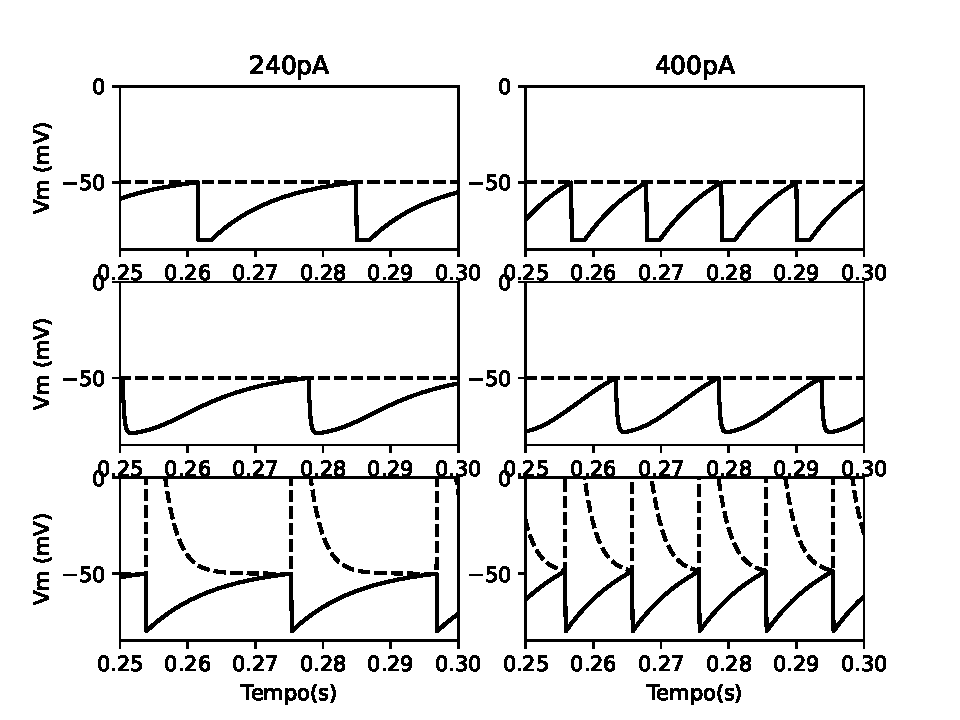
\includegraphics[width=0.7\linewidth]{figs/lif_refratario}
	\end{figure}
	
\end{description}

\subsubsection{Adaptação da taxa de disparo}
\begin{itemize}
	\item Uma diminuição da taxa de disparos de potenciais de ação logo após o primeiro disparo
	\item É implementada de maneira semelhante ao método da condutância refratária para o período refratário, porém com duas diferenças:
	\begin{itemize}
		\item O incremento da condutância é menor em comparação ao do período refratário. Esse incremento menor não impede o disparo de novos potenciais, como no período refratário, porém diminui a taxa deles
		\item A escala de tempo (a constante) da condutância adaptativa é bem maior, o que permite o acúmulo das condutâncias ao longo da sequência de disparos
	\end{itemize}
\end{itemize}

\begin{figure}[htb!]
	\centering
	\caption{Adaptação da taxa de disparo no neurônio LIF}
	\label{fig:lifatd}
	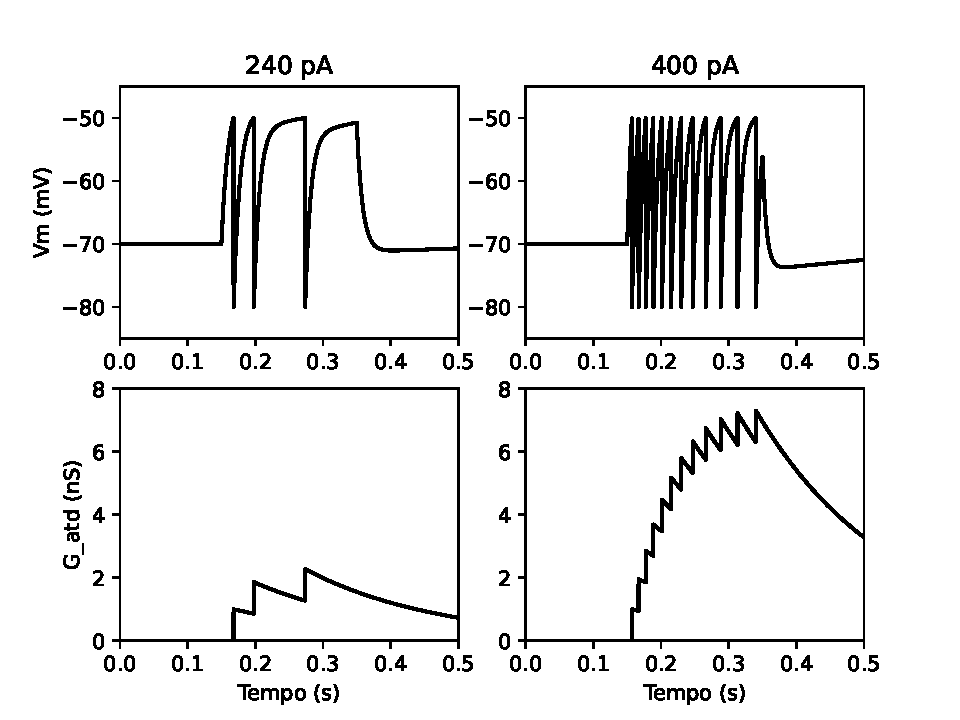
\includegraphics[width=0.7\linewidth]{figs/lif_atd}
\end{figure}

\subsubsection{Modelo LIF exponencial}
\begin{itemize}
	\item Incorpora um termo adicional para a geração do potencial de ação
	\item Não há exatamente um valor fixo para o disparo do potencial, e sim um intervalo ($\Delta_{th}$)
	\item O termo exponencial acrescenta uma corrente despolarizante, elevando quase que instantaneamente o valor do potencial de membrana quando este se aproxima do limiar
	\item O crescimento tende ao infinito, porém nas simulações é definido um limite ($V_{max}$) devido o computador ter problemas para lidar com valores infinitos
\end{itemize}
$$
c_m\frac{dV_m}{dt} = G_L(E_L-V_m) + G_L\Delta_{th}\exp\Big(\frac{V_m-V_{th}}{\Delta_{th}}\Big) + I_{ap}
$$$$
\text{se } V_m > V_{max} \text{ então } V_m\mapsto V_{reset}
$$

\begin{figure}[htb!]
	\centering
	\caption{Comparação dos modelos LIF e ELIF}
	\label{fig:elif}
	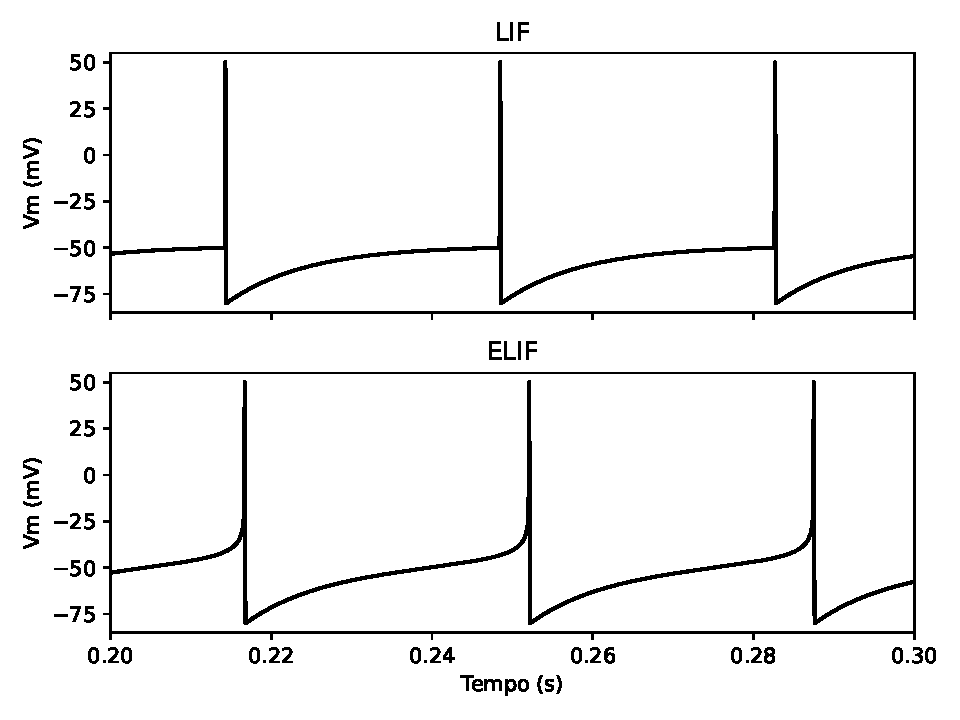
\includegraphics[width=0.7\linewidth]{figs/elif}
\end{figure}


\subsubsection{Modelo LIF exponencial adaptativo}
\begin{itemize}
	\item Adiciona uma corrente adaptativa hiperpolarizante, que depende do potencial de membrana
	\item É um modelo com duas equações. A primeira contém a dinâmica do potencial de membrana (semelhante ao modelo anterior), e a segunda é referente à adaptação ($w$)
	\item Ambas são resetadas quando ocorre um potencial de ação
	\item É capaz de descrever padrões de disparo comuns (\textit{bursting, fast spiking, regular spiking,} etc)
\end{itemize}
$$
c_m\frac{dV_m}{dt} = G_L(E_L-V_m) + G_L\Delta_{th}\exp\Big(\frac{V_m-V_{th}}{\Delta_{th}}\Big) - w + I_{ap}
$$$$
\tau_w\frac{dw}{dt}=a(V_m-E_L)-w
$$$$
\text{se } V_m > V_{max} \text{ então } V_m\mapsto V_{reset} \text{ e } w\mapsto w + b
$$
sendo $a$ o parâmetro de agrupamento e $b$ o de adaptação.

\begin{figure}[h!]
	\centering
	\caption[Resposta do modelo AELIF]{Resposta do modelo AELIF para um pulso de corrente de 1 $nA$. Em cima, o potencial de membrana. Embaixo, a variável de adaptação}
	\label{fig:adexrs}
	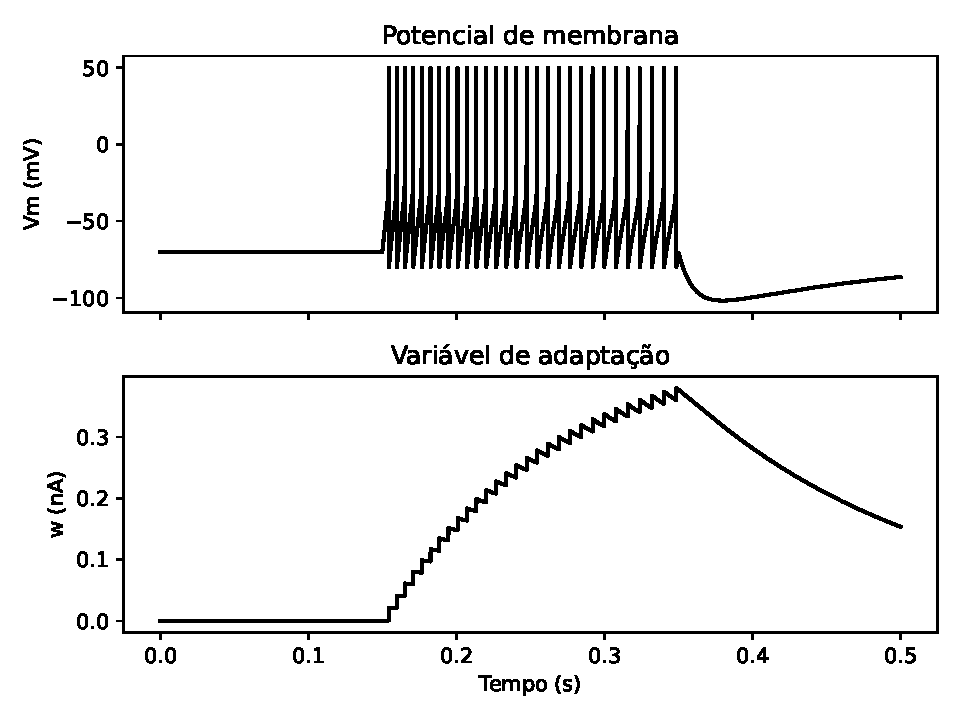
\includegraphics[width=0.7\linewidth]{figs/aelif}\\
\end{figure}


\subsection{Modelo de Izhikevich}\label{sec:izhikevich}

\subsection{Modelo de Hodgkin-Huxley}\label{sec:modelohh}
\subsubsection{Canais iônicos}
\cite{miller_introductory_2018}
\begin{description}
	\item[Canal iônico dependentes de tensão] A probabilidade de abertura do canal é modificada em função do potencial de membrana
	\item[Ativação] O processo de abertura de um canal iônico, geralmente devido à despolarização. O seu oposto é a \textbf{desativação}. A despolarização aumenta a probabilidade de um canal estar aberto
	\item[Inativação] O processo que impede a abertura dos canais. O seu oposto, necessário para que o canal se abra, é a \textbf{desinativação}
	\item[Variável de portão] Uma variável com valores entre 0 e 1, representando a fração de canais iônicos em um determinado estado (ativado/desativado, inativado/desinativado)
\end{description}

\begin{figure}[htb!]
	\centering
	\caption{Mecanismo de funcionamento dos canais iônicos dependentes de tensão}
	\label{fig:canais}
	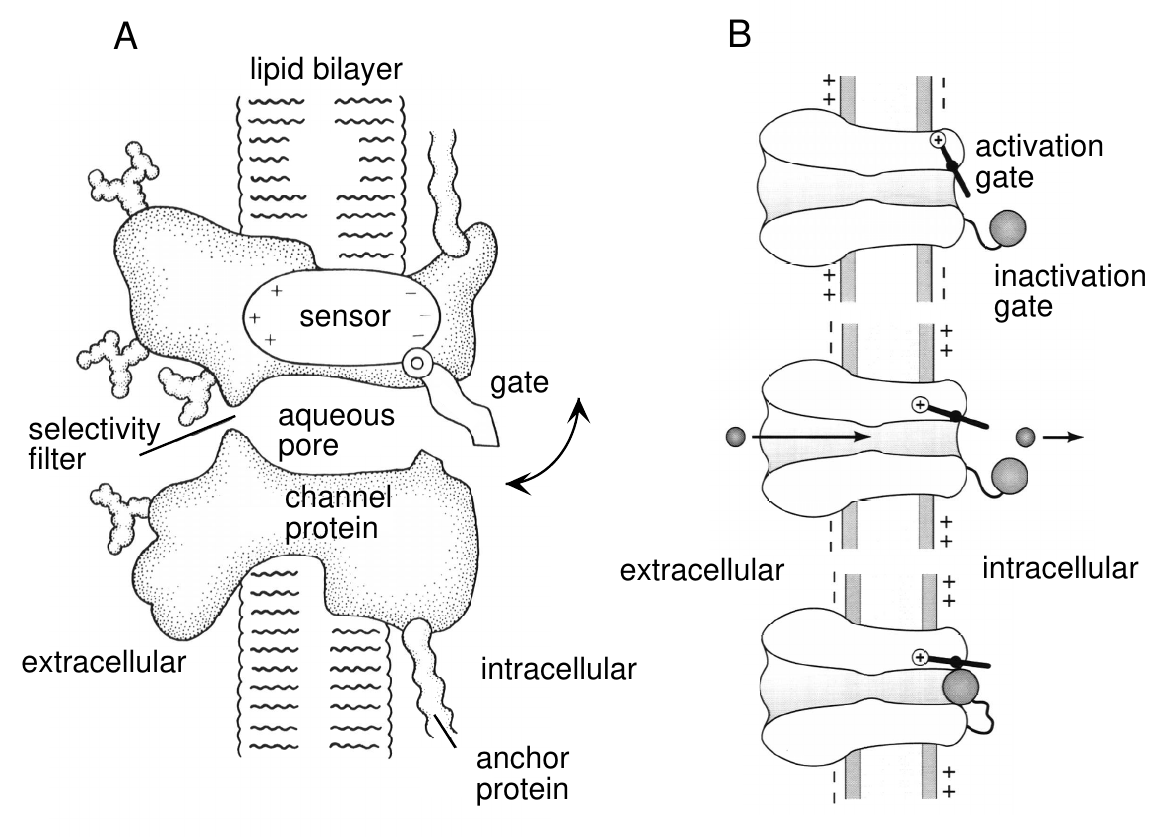
\includegraphics[width=0.6\linewidth]{figs/canais}\\
	\small{Fonte: \cite{dayan_theoretical_2001}}
\end{figure}


%%% nome de alguma outra sub-seção
No modelo de Hodgkin-Huxley o potencial de membrana é dado pela equação abaixo:
$$
C_m\frac{dV_m}{dt}=G_L(E_L-V_m)+G_{Na}^{(max)}m^3h(E_{Na}-V_m)+G_K^{(max)}n^4(E_K-V_m)+I_{ap}
$$
que é semelhante à equação do modelo LIF, porém com dois elementos a mais, um para a condutância dependente de tensão de sódio e outra para a de potássio. Essas elementos incluem as variáveis de portão: \textbf{m} para ativação de sódio, \textbf{h} para inativação de sódio, e \textbf{n} para ativação de potássio. Cada variável segue sua própria dinâmica, definidas nas equações diferenciais abaixo:
$$
\frac{dm}{dt}=\alpha_m(1-m)-\beta_mm
$$$$
\frac{dh}{dt}=\alpha_h(1-h)-\beta_hh
$$$$
\frac{dn}{dt}=\alpha_n(1-n)-\beta_nn
$$
sendo $\alpha$ a constante de crescimento de cada variável, e $\beta$ a constante de decrescimento, ambas também dependentes de tensão, conforme as equações abaixo:
$$
\alpha_m=\frac{10^5(-V_m-0.045)}{\exp[100(-V_m-0.045)]-1}
\qquad
\beta_m=4*10^5\exp\Big[\frac{(-V_m-0.070)}{0.018}\Big]
$$$$
\alpha_h=70\exp[50(-V_m-0.070)]
\qquad
\beta_h=\frac{10^3}{1+\exp[100(-V_m-0.040)]}
$$$$
\alpha_n=\frac{10^4(-V_m-0.060)}{\exp[100(-V_m-0.060)]-1}
\qquad
\beta_n=125\exp\Big[\frac{(-V_m-0.070)}{0.08}\Big]
$$
As variáveis de portão também podem se definidas pelas suas equações em \textbf{regime permanente} (o comportamento em repouso depois de um longo período de tempo): \cite{ermentrout_mathematical_2010}
$$
m_\infty=\frac{\alpha_m}{\alpha_m+\beta_m}
\qquad
h_\infty=\frac{\alpha_h}{\alpha_h+\beta_h}
\qquad
n_\infty=\frac{\alpha_n}{\alpha_n+\beta_n}
$$
com as respectivas constantes de tempo:
$$
\tau_m=\frac{1}{\alpha_m+\beta_m}
\qquad
\tau_h=\frac{1}{\alpha_h+\beta_h}
\qquad
\tau_n=\frac{1}{\alpha_n+\beta_n}
$$
O modelo também assume algumas constantes além das usadas em outros modelos:
\begin{description}
	\item[Condutância máxima de sódio ($G_{Na}^{(max)}$)] $12\mu S$
	\item[Condutância máxima de potássio ($G_K^{(max)}$)] $3,6\mu S$
	\item[Potencial de reversão do sódio ($E_{Na}$)] $45mV$
	\item[Potencial de reversão do potássio ($E_K$)] $-82mV$
\end{description}

\begin{figure}[h!]
	\centering
	\caption{Potencial de membrana gerado pelo modelo de Hodgkin-Huxley}
	\label{fig:hhvm}
	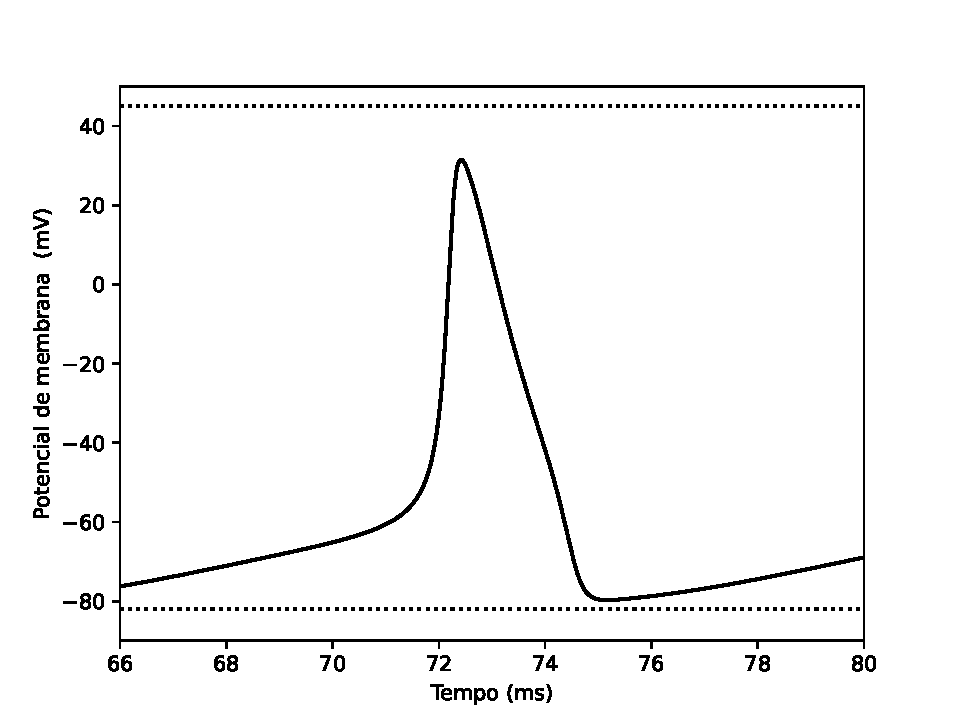
\includegraphics[width=0.7\linewidth]{figs/hh_vm}
\end{figure}

\begin{figure}[htb!]
	\centering
	\caption{Dinâmica das variáveis de portão}
	\label{fig:portoes}
	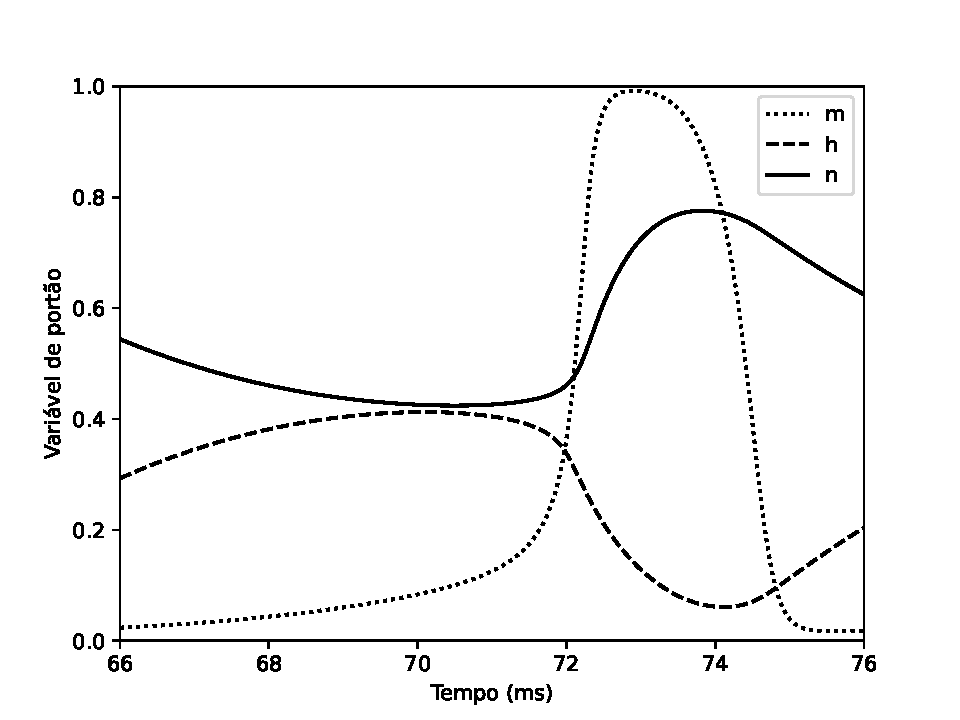
\includegraphics[width=0.7\linewidth]{figs/portoes}
\end{figure}
\section{Modelos de taxa de disparo}\label{sec:modelostaxa}
